%!TEX root = /Users/domaubert/Documents/Lectures/cosmologie/cosmo_main.tex

\chapter{Dynamique de l'Univers Homogène}
Nous savons dorénavant que la distance physique \index{distance!physique} $r$ entre deux points dans l'Univers peut évoluer au cours du temps, suivant une simple loi d'échelle:
\begin{equation}
r(t)=a(t)r_0
\end{equation}
où $r_0$ désigne la distance actuelle entre 2 points\sidenote{appelée aussi distance comobile\index{distance!comobile}}. La facteur sans dimension $a(t)$ encode toute la dépendance temporelle de l'évolution des distances dans l'Univers homogène. Reste à présent à déterminer l'évolution temporelle de ce facteur $a(t)$, appelé aussi \textit{facteur} ou \textit{paramètre} d'expansion \index{facteur d'échelle}\sidenote{appelé aussi facteur d'échelle}.
En particulier l'un des objectif est de parvenir à comprendre l'histoire observée de notre Univers avec un Big-Bang\index{Big-Bang} ($a\rightarrow 0$ quand $t\sim 0$), des distances qui augmentent avec le temps ($\dot a>0$) et une expansion\index{expansion} récente accélérée ($\ddot a>0$ quand $t\sim t_0$).

\section{Fluides Cosmologiques}

\begin{figure}[htbp]
	\centering
		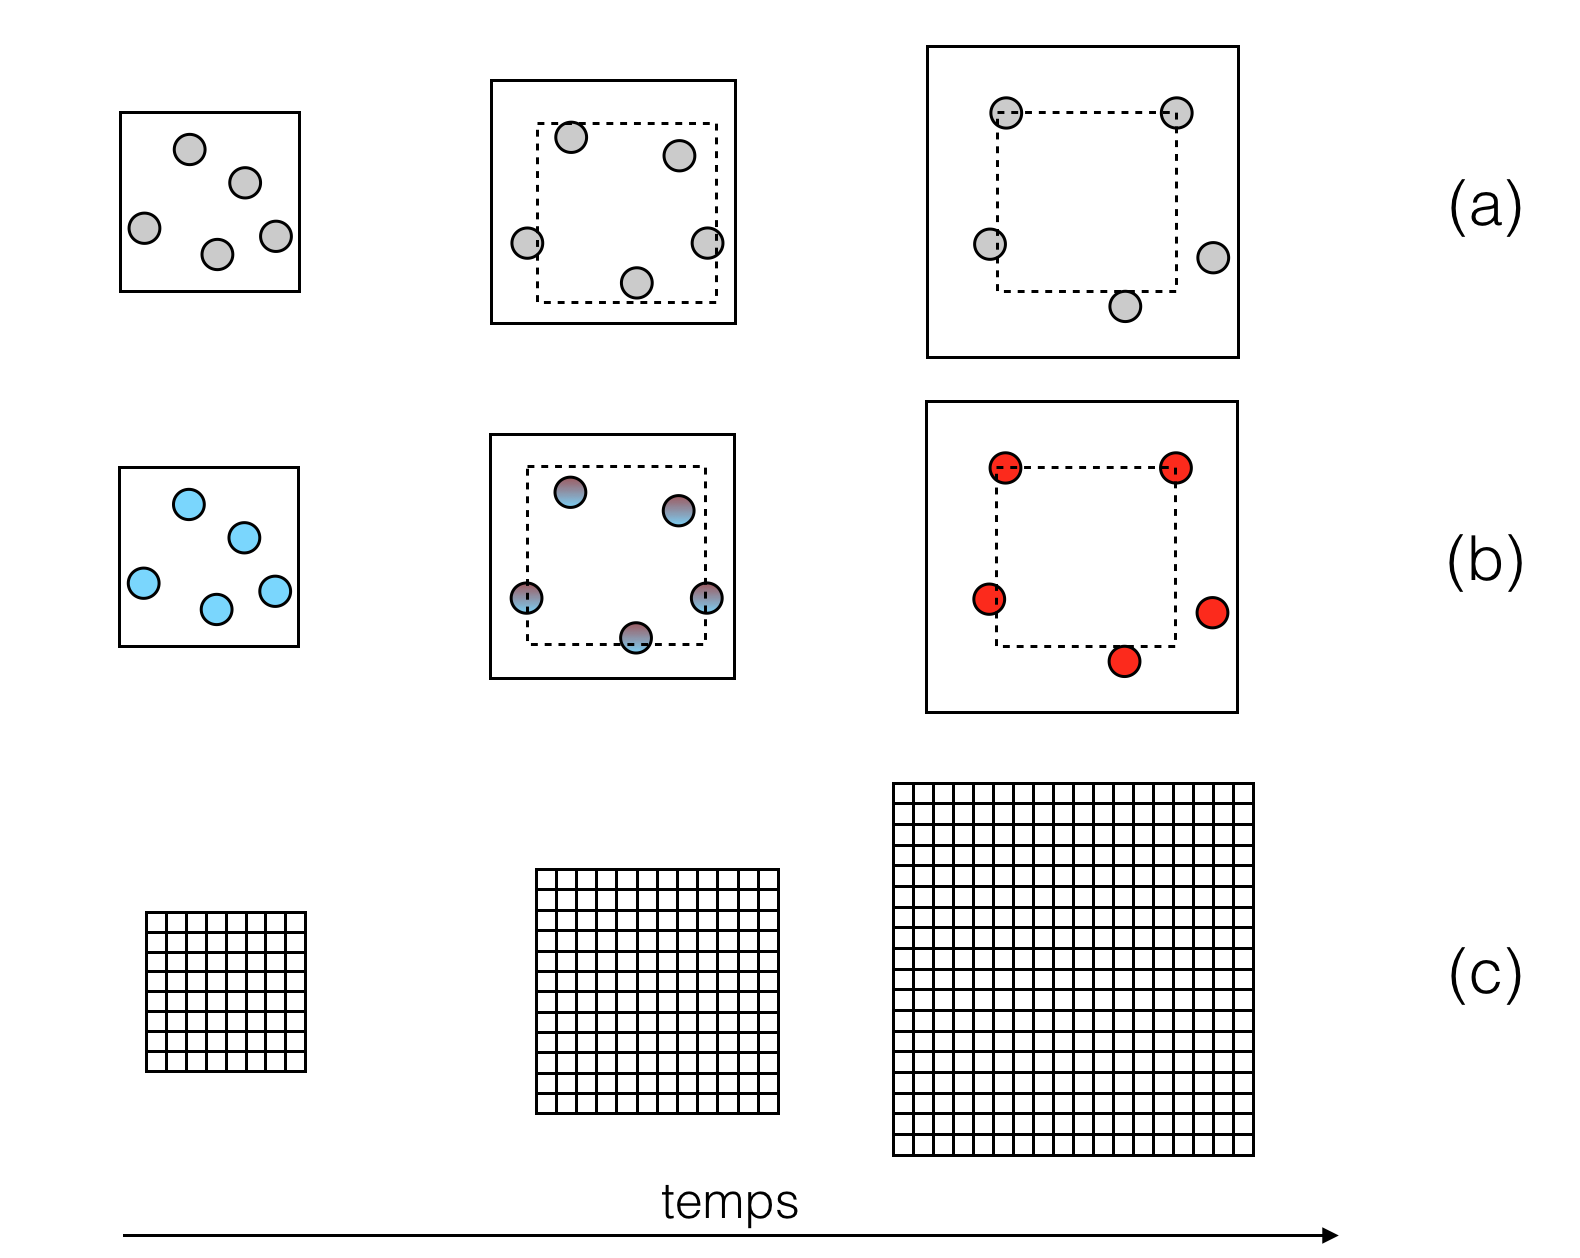
\includegraphics[height=10cm]{figs/fluides.png}
	\caption[Evolution des fluides cosmologiques]{Evolution schématique des 3 fluides cosmologiques sous l'effet de l'expansion. Pour la matière non-relativiste (a), le nombre de particules reste constant, l'énergie totale est constante et la densité d'énergie diminue avec le volume. Pour la matière relativiste (b), le nombre de particules reste constant mais l'énergie individuelle de chacune diminue sous l'effet du rougissement cosmologique: l'énergie totale diminue et la densité d'énergie diminue sous le double effet du rougissement et de la dilution. Pour le 'volume' (c), la densité d'énergie est constante dans chaque élément de volume (représenté par une case) et l'énergie totale à l'intérieur du volume de contrôle augmente avec l'expansion.}
	\label{f:fluides}
\end{figure}

On désigne par \textit{fluides} les différentes formes sous lesquelles l'énergie-impulsion se trouve stockée dans l'Univers. Ces fluides\index{fluide cosmologique} opèrent comme termes  sources de l'équation de Friedmann (Eq. \ref{e:friedmann}) et régissent donc la dynamique de l'espace-temps. 

Ces fluides sont supposés isotropes et parfaits (non visqueux): leurs pressions se résument donc à des scalaires comme pour un fluide "standard". Par la suite on distinguera 3 types de fluides cosmologiques:
\begin{itemize}
\item la \textit{matière} qui désigne plus précisément la matière non-relativiste et qui se distinguera par une pression négligeable,
\item le \textit{rayonnement} qui désigne par abus de langage toute forme de matière relativiste \sidenote{dont les photons et les neutrinos\index{neutrino} par exemple}. Sa pression est non nulle,
\item le \textit{volume} qui désigne une forme d'énergie dont la densité volumique est constante. Comme expliqué par la suite, on parle aussi de \textit{vide}.
\end{itemize}
Ces 3 fluides cosmologiques sont définis par des densités d'énergie et des pressions dont les comportements diffèrent, notamment en fonction du paramètre d'expansion $a$. Par la suite, on pourra démontrer que leurs contributions à l'histoire de la dynamique de l'Univers vont se faire à différentes époques et suivant différentes dépendances temporelles.

Afin de comprendre leurs influences respectives sur la dynamique du cosmos, la procédure à suivre sera toujours plus ou moins identique. Rappelons l'expression de l'équation de Friedmann\index{equation de Friedmann@équation de Friedmann}
\begin{equation}
\frac{\ddot a}{a}=-\frac{4\pi G}{3c^2}(\rho c^2 +3 P).
\end{equation}
Nous voyons que la dépendance temporelle de $a(t)$ (décrite par le membre de gauche de l'équation) est 'sourcée' par les quantités du membre de droite qui caractérisent la matière contenue dans l'Univers.
Pour intégrer cette équation et trouver une expression pour $a(t)$, il s'agit donc de connaitre la densité d'énergie\index{densité!d'énergie} du fluide cosmologique ainsi que la pression qui l'accompagne: ces quantités constituent les \textit{sources} de la variation de $a$ et donc de la dynamique des distances dans l'Univers. 

Notons que dans le cas général, $\rho=\rho(t)=\rho(a)$ et $P=P(t)=P(a)$. Le terme source va donc varier au cours du temps (ou de façon équivalente en fonction de la valeur du facteur d'expansion), et va donc modifier le comportement de $a(t)$. Si jamais plusieurs fluides se trouvent être présents simultanément, chacun aura sa propre contribution au terme source de l'équation de Friedmann dont l'expression devient alors:
\begin{equation}
\frac{\ddot a}{a}=-\frac{4\pi G}{3c^2}\sum_i^\mathrm{fluides}(\rho_i c^2 +3 P_i).
\end{equation}

Généralement, la densité d'énergie $\rho_i c^2$ est facilement obtenue en faisant un bilan du nombre de particules du fluide considéré. Ici le fluide est considéré comme libre \sidenote{sans influence exercée par une force extérieure}, non-soumis à une interaction extérieure, et chacun de ses éléments emmène une énergie:
\begin{equation}
E^2=p^2c^2+m^2c^4,
\end{equation}
constitué de son énergie cinétique et de son énergie de masse\index{energie@énergie!cinétique} \index{energie@énergie!masse}.

La pression nécessite généralement un peu plus d'effort. Afin d'évaluer cette pression\index{pression}, une approche consiste à considérer que la \textit{variation} d'énergie interne avec le volume est due au travail\index{travail} des forces de pression. Ainsi si on considère un volume de contrôle que l'on fait varier d'une quantité $dV$, la variation interne d'énergie est proportionnelle à cette pression:
\begin{equation}
dE=-PdV,
\label{e:therm1}
\end{equation}
il ne s'agit ni plus ni moins que d'une application du premier principe de la thermodynamique\sidenote{appliqué ici en l'absence de flux de chaleur, qui est nul dans un Univers homogène}. En cosmologie, la source de variation du volume d'un contour est la dynamique de l'Univers, via le facteur d'expansion. Ainsi le volume $V$ mesuré à n'importe quel instant peut être exprimé en fonction du volume mesuré aujourd'hui, $V_0$, du même contour:
\begin{equation}
V=V_0a^3,
\end{equation}
d'où l'expression suivante pour la variation $dV$
\begin{equation}
dV=V_03a^2da=3V\frac{da}{a}.
\label{e:dV}
\end{equation}
Notons par exemple que le taux de variation du volume est donné par:
\begin{equation}
\frac{dV}{dt}=3HV
\end{equation}
et fait intervenir la fonction de Hubble, $H(a)=\dot a/a$\index{Hubble!fonction}.

\subsection{La matière non-relativiste}
Le premier fluide considéré est la matière non-relativiste, celle qui nous est la plus familière. On y trouve les baryons\index{baryons} et toute forme de matière noire froide\index{matière noire!froide}\sidenote{\textit{froid} désigne ici un fluide dont les particules sont animées de faibles vitesses devant $c$, voir le chapitre dédié à la matière noire}. Cette matière se caractérise par une énergie par particule dominée par l'énergie de masse\index{energie@énergie!masse} et une énergie cinétique \index{energie@énergie!cinétique}négligeable devant cette dernière ($pc\ll mc^2$)~:
\begin{equation}
E\sim mc^2.
\end{equation}
Supposons un volume de contrôle $V$ à l'intérieur duquel se trouve $N$ particules non-relativistes (voir Fig. \ref{f:fluides} (a)). A l'intérieur, la densité d'énergie vaut:
\begin{equation}
\rho_m c^2=\frac{Nmc^2}{V}=\frac{Nmc^2}{a^3V_0}=\rho_{m0}c^2\frac{1}{a^3}.
\label{e:densm}
\end{equation}
Ici la masse d'une particule est supposée constante et le volume de contrôle contient toujours le même nombre de particules. Cette dernière hypothèse revient à considérer qu'il n'y a aucune création ou destruction nette de particules et que le flux net au travers de la surface délimitant ce volume est nul \sidenote{voir aussi le chapitre dédié au modèle newtonien de cosmologie}: pour un Univers homogène, donc sans variations spatiales susceptibles de générer des mouvements de matière, cette dernière hypothèse est raisonnable. L'équation \ref{e:densm} nous renseigne sur l'évolution temporelle de la densité d'énergie de la matière non-relativiste. Dans un Univers en expansion, $a$ est une fonction croissante du temps :  on constate alors que cette densité diminue au cours du temps, par simple dilution d'un nombre constant de particules (et donc d'énergie totale) dans un volume de plus en plus grand. Toujours dans le cas d'un facteur d'expansion croissant avec le temps, on constate que la densité d'un tel fluide était plus importante dans le passé.

Qu'en est-t-elle de la pression de ce fluide non relativiste ? Si l'on met à profit l'équation \ref{e:therm1}, on obtient:
\begin{equation}
P_m=-\frac{dE_m}{dV}
\end{equation}
où $E_m$ est l'énergie totale dans le volume de contrôle considéré. Dans le cas présent cette énergie est complètement dominée par l'énergie de masse, qui est constante dans ce volume, y compris lorsque le volume est modifié par la dynamique de l'Univers. Par conséquent, pour un fluide non-relativiste, la pression est considérée comme négligeable:
\begin{equation}
P_m=0.
\end{equation}
Ceci n'est pas une totale surprise: en effet nous avons défini ce fluide non-relativiste comme étant \textit{absolument froid}, i.e. avec une contribution nulle (en pratique négligeable) de l'énergie cinétique à son énergie interne totale \sidenote{la température est une mesure de la dispersion de vitesse : être 'froid' implique donc une faible contribution de l'énergie cinétique, voir le chapitre dédié à la matière noire}. Pour mémoire, la pression est une manifestation des mouvements microscopiques des particules individuelles: celles-ci étant figées, il en résulte une pression égale à zéro.

\subsection{La Matière Relativiste}
On désigne par matière relativiste\index{matière relativiste} toute forme de matière pour laquelle la contribution de son énergie cinétique domine celle de son énergie de masse. Pour une particule de ce fluide, nous avons $mc^2\ll pc$ et son énergie individuelle est donnée par:
\begin{equation}
E\sim pc,
\end{equation}
où $p$ désigne l'impulsion de la particule. Cela concerne bien évidemment les photons mais également toute particule très légère comme les neutrinos\index{neutrinos}. Supposons le même volume de contrôle que pour la matière non relativiste, avec une densité $N$ de particules chacune porteuse d'une énergie $pc$ (voir Fig. \ref{f:fluides} (b)). Comme précédemment, la densité d'énergie de ce volume de contrôle est donnée par:
\begin{equation}
\rho_rc^2=\frac{Npc}{V}.
\end{equation}
Toutefois, contrairement à la masse, l'impulsion est sensible à la dynamique de l'Univers puisqu'elle peut s'exprimer en fonction de la longueur d'onde qui elle-même subit les effets de rougissement cosmologique\sidenote{on rappelle que le redshift $z$\index{redshift} est relié au facteur d'expansion via $a=\frac{1}{1+z}$}:
\begin{equation}
p=\frac{hc}{\lambda}=\frac{hc}{a\lambda_0}=\frac{p_0}{a}=p_0(1+z).
\end{equation}
Il en résulte une dépendance temporelle de la densité d'énergie relativiste qui est différente de celle trouvée précédemment pour la matière non-relativiste~:
\begin{equation}
\rho_rc^2=\frac{Np_0c}{ a^4 V_0}=\rho_{r0}c^2\frac{1}{a^4}.
\end{equation}
Comparée à la matière non-relativiste, la densité d'énergie varie ici plus rapidement (et baisse plus rapidement si $a$ croît avec le temps). La raison est simple~: en plus de l'effet de dilution géométrique s'ajoute une baisse de l'énergie individuelle portée par chaque particule à cause du rougissement cosmologique.

Calculons maintenant la pression \index{pression} comme taux de variation de l'énergie totale avec le volume:
\begin{equation}
P_r=\frac{dE_r}{dV}=-\frac{d(Npc)}{dV}.
\end{equation}
Grâce à l'équation \ref{e:dV} la pression peut être réexprimée en fonction de la densité d'énergie:
\begin{equation}
P_r=Nc\frac{d(p)}{dV}=Nc\frac{dp}{da}\frac{da}{dV}=-Nc\frac{-p_0}{a^2}\frac{a}{3V}=\frac{1}{3}\rho_rc^2.
\end{equation}
Dans ce cas la pression est non nulle et est une fonction simple de la densité d'énergie. A nouveau cela n'est pas une surprise puisque nous avons défini ces particules comme ne possédant qu'une énergie cinétique, qui est la source de pression.

\subsection{Le "Volume"}
De prime abord, le dernier type de fluide est de nature hypothétique et est \textit{défini} par une densité d'énergie constante:
\begin{equation}
\frac{dE_v}{dV}=\Lambda=\mathrm{const.}
\end{equation}
On appellera ce fluide "volume" car il ne repose pas sur l'existence d'une particule le composant mais davantage sur une quantité d'énergie qu'apporte nécessairement un volume donné. Remarquons que si le volume de contrôle augmente (sous l'effet d'un facteur d'expansion croissant par exemple), la quantité d'énergie présente dans ce volume de contrôle augmente aussi (voir Fig. \ref{f:fluides} (c)).  On parle aussi d'énergie du "vide"\index{energie@énergie!vide}, puisqu'une telle énergie est présente y compris en l'absence de matière ou de rayonnement.

Compte tenu de cette définition, la densité d'énergie ne varie pas au cours du temps et vaut:
\begin{equation}
\rho_vc^2=\rho_{v0}c^2,
\end{equation}
tandis que la pression vaut
\begin{equation}
P_v=-\frac{dE_v}{dV}=-\rho_vc^2.
\end{equation}
On constate qu'un tel type de contribution énergétique produit une pression \textit{négative}. A l'inverse du comportement d'un fluide standard, son énergie interne augmente avec son volume, le 'vide' ne subit pas de détente \sidenote{habituellement c'est l'inverse : un gaz chauffe quand on le comprime, son énergie interne augmente quand le volume diminue.}. Cela résulte de la non-variation de la densité d'énergie à l'intérieur du volume de contrôle même si celui-ci évolue sous l'effet du facteur d'expansion.

A nouveau ce fluide est une hypothèse de travail. Toutefois il s'avère que ce type de fluide exotique permet une bonne représentation de la dynamique \textit{observée} des distances dans l'Univers. Ce fluide est la fameuse \textit{énergie noire}\index{energie noire@énergie noire}, dont la nature nous échappe complètement actuellement et qui permet de rendre compte de l'accélération\index{accélération!expansion} observée de l'expansion de l'Univers. La densité d'énergie étant constante dans le temps et dans l'espace, on parle aussi de \textit{constante cosmologique} \index{constante cosmologique}.

\section{Epoques de domination}
\begin{figure}[htbp]
	\centering
		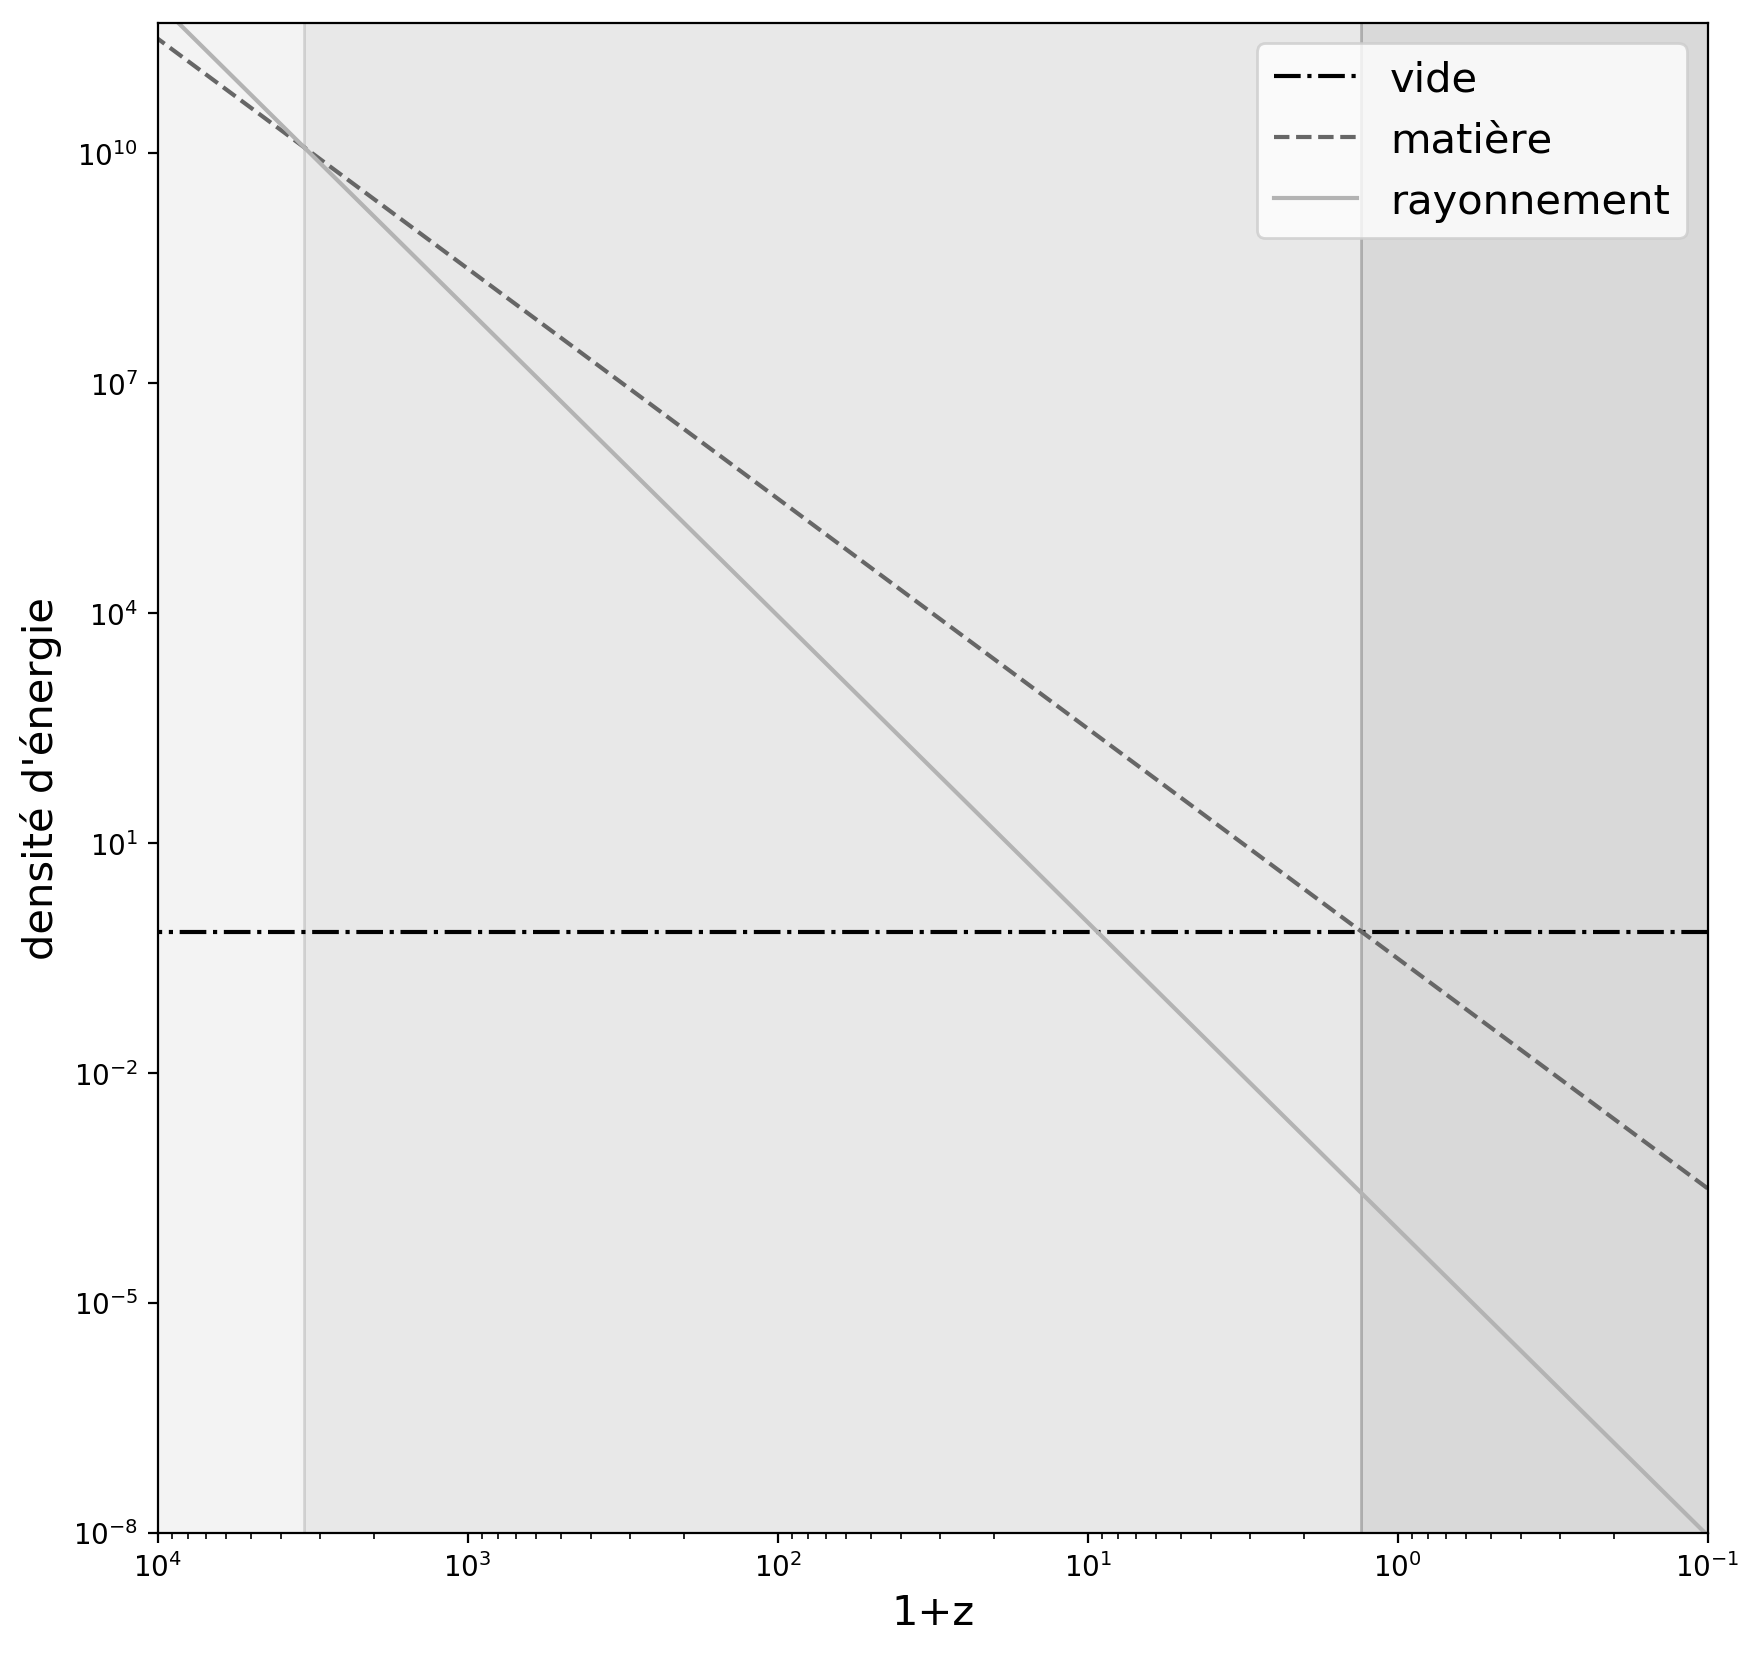
\includegraphics[height=10cm]{figs/era.png}
	\caption[Epoques de domination des fluides cosmiques]{Evolution temporelle de la densité d'énergie des 3 fluides cosmologiques pour une cosmologie standard ($\Omega_m \sim 0.31$, $\Omega_v \sim 0.69$ et $\Omega_r\sim 9.1\times 10^{-5}$, Planck 2015). Le temps s'écoule de la gauche vers la droite, l'époque actuelle correspondant à $1+z=1$. Les 3 époques de dominations successives sont celles du rayonnement, de la matière et du vide. La première transition, entre rayonnement et matière est \textit{ l'équivalence}, avec $z_e\sim 3371$ et la seconde, vers un Univers dominé par l'énergie du vide, prend place vers $z_v \sim 0.3$. }
	\label{f:era}
\end{figure}
Le bilan des trois fluides étudiés est donné dans la table suivante. On notera qu'on utilise la nomenclature standard des trois fluides: "matière" pour la matière non relativiste\index{matière!non relativiste}, "rayonnement" pour la matière relativiste\index{matière!relativiste} et "vide" pour l'énergie de volume.
\begin{table}[h]
\begin{center}
\begin{tabular}{|c|c|c|c|}
\hline 
 & Caractéristique & Densité d'énergie & Pression \\ 
\hline 
Matière & $E\sim mc^2$ & $\rho_mc^2 =a^{-3}\rho_{m0}c^2$& $P_m=0$\\ 
\hline 
Rayonnement & $E\sim pc$ & $\rho_rc^2 =a^{-4}\rho_{r0}c^2$ & $P_r=\rho_rc^2/3$ \\ 
\hline 
Vide & $dE/dV\sim \mathrm{cst}$ & $\rho_vc^2 =\rho_{v0}c^2$ & $P_v=-\rho_vc^2$ \\ 
\hline 
\end{tabular} 
\end{center}
\caption{Les 3 fluides cosmologiques}
\end{table}

En réinjectant ces résultats dans l'équation de Friedmann (eq. \ref{e:friedmann})  on obtient une expression détaillée du terme source qui permet déjà d'entrevoir certaines caractéristiques de la dynamique des distances dans l'Univers:
\begin{equation}
\frac{\ddot a}{a}=-\frac{4\pi G}{3}(\frac{\rho_{m0}}{a^3}+2\frac{\rho_{r0}}{a^4}-2\rho_{v0}).
\label{e:esource}
\end{equation}
Dans un premier temps, il apparaît que la matière et le rayonnement ont un même effet qualitatif et tendent à décélérer la variation du facteur d'expansion (en imposant $\ddot a<0$). Cette décélération\index{décélération!expansion} est d'autant plus faible que les distances  sont grandes (i.e. $\ddot a \rightarrow 0$ quand $a$ augmente) et que les densités d'énergies associées sont faibles, permettant d'anticiper sur une sorte de "régulation". A l'inverse, le "vide" produit une accélération\index{accélération!expansion} de la variation de $a$ (avec $\ddot a>0$)~: cela résulte du terme de pression négative\index{pression} qui produit une contribution nette positive de ce fluide au terme source de l'équation de Friedmann. Notons que cette contribution reste constante au cours du temps, avec $\ddot a$ augmentant avec $a$ \sidenote{en effet nous avons $\ddot a\sim \rho_{v0} a$. Plus $a$ augmente, plus sa croissance accélère et devient 'incontrôlée'}, indiquant dès à présent un effet "catastrophique" non régulé. 

Enfin on constate que les contributions au terme source de l'équation de Friedmann ont des dépendances temporelles différentes en fonction du fluide considéré (voir Fig. \ref{f:era}). En supposant une évolution de $a$ croissante au cours du temps, il apparaît qu'entre le rayonnement (qui varie en $a^{-4}=(1+z)^4$) et la matière (qui varie en $a^{-3}=(1+z)^3$), la première domine\index{domination!période} aux époques qui correspondent aux faibles valeurs de $a$ (donc généralement au début) tandis que la matière doit prendre le dessus aux plus grandes valeurs du facteur d'expansion (donc généralement plus tard). Il existe donc une époque où ces deux fluides ont exactement la même densité d'énergie~: cette époque est appelée \textit{l'époque d'équivalence} \sidenote{l'équivalence est en place pour $z\sim 3000$}. Avant l'équivalence, la matière relativiste domine. Après l'équivalence, la matière non-relativiste dicte la dynamique de l'Univers.

Mais qu'en est-il de la densité d'énergie du vide, dont la valeur est par définition constante? Le verdict est sans appel: compte tenu du fait que les densités d'énergie des deux autres fluides sont des fonctions décroissantes de $a$, il existe \textit{toujours} une valeur seuil du paramètre d'expansion au delà de laquelle le vide domine \sidenote{cette transition a eu lieu il y a environ 3 milliards d'années, pour $z\sim0.3$}. Tout modèle d'Univers avec une énergie du vide finira par être dominé par cette dernière, pour peu que l'on attende suffisamment longtemps.

Pour finir, disons clairement que les relations obtenues entérinent la non-conservation\index{conservation!énergie} de l'énergie totale du Cosmos. Pour un Univers dominé par une énergie du vide de densité d'énergie constante, l'expansion implique nécessairement des volumes croissants et donc une énergie totale croissante.  Même en l'absence de ce fluide inconnu, le rougissement individuel des photons fait que l'énergie totale stockée dans la matière relativiste doit décroître : la densité d'énergie varie en $a^{-4}$ et le volume en $a^3$ conduisant à une énergie totale non constante, inversement proportionnelle à $a$. Seul un Univers contenant uniquement de la matière non-relativiste, par conservation du nombre de particules d'énergie constante, garantit à priori une conservation de l'énergie totale : cet Univers n'est toutefois pas le nôtre qui contient à minima du rayonnement en plus de cette matière. Rappelons que cette non-conservation n'est pas problématique : la relativité générale ne garantit pas de façon générale la conservation du scalaire 'énergie' mais propose une relation plus complexe, plus générale sur le \textit{tenseur} énergie-impulsion \sidenote{voir aussi le chapitre sur les fondamentaux}. Par ailleurs, on peut se souvenir que la conservation de l'énergie est une traduction de l'invariance\index{invariance} par translation temporelle du résultat d'une expérience donnée\sidenote{de même que l'invariance par translation spatiale implique une conservation de l'impulsion ou l'invariance par rotation implique une conservation du moment cinétique} : dans un Univers où la géométrie possède une évolution, cette invariance n'est bien sûr pas garantie.

\subsection{Paramètre de densité $\Omega$}

A ce stade il nous faut introduire une nouvelle expression, le paramètre de densité $\Omega$\index{paramètre!densité}, qui apparaît naturellement lorsque l'on intègre l'équation \ref{e:esource}. Cette intégration se fait naturellement en multipliant l'équation \ref{e:esource} par $2\dot a a$, qui permet d'obtenir:
\begin{equation}
\left(\frac{\dot a}{a}\right)^2=H(a)^2=\frac{8\pi G}{3}(\frac{\rho_{m0}}{a^3}+\frac{\rho_{r0}}{a^4}+\rho_{v0}-\frac{k}{a^2}).
\end{equation}
Notez l'introduction d'une constante d'intégration $k$ que nous discuterons par la suite. Le terme de gauche n'est autre que le carré de la fonction de Hubble\index{Hubble!fonction} au cours du temps: aussi pour des raisons de symétrie, il est tentant de multiplier le terme de droite par $H_0$, ce qui permet d'écrire:
\begin{equation}
H^2=H_0^2(\frac{\Omega_m}{a^3}+\frac{\Omega_r}{a^4}+\Omega_v-\frac{\Omega_k}{a^2}).
\label{e:hubblea}
\end{equation}
C'est cette équation qu'il faudra intégrer par la suite pour obtenir l'évolution temporelle du facteur d'échelle $a$ et elle introduit les paramètre de densités (dans l'ordre) de la matière, du rayonnement, du vide et de la constante d'intégration. Ces quantités sont sans dimension et égales à:
\begin{equation}
\Omega=\frac{\rho_0 c^2}{\rho_c c^2},
\end{equation}
où $\rho_c$ désigne la \textit{densité critique}\index{densité critique} dont l'expression est donnée par\sidenote{notons que l'on retrouve les grandeurs obtenus dans le chapitre dédié à la cosmologie Newtonienne}:
\begin{equation}
\rho_c=\frac{3H_0^2}{8\pi G}.
\end{equation}
Les paramètres de densités sont donc l'expression des densité d'énergie \textit{mesurées aujourd'hui} des différents fluides en unités de cette densité critique.

Si l'on applique l'équation \ref{e:hubblea} aujourd'hui quand $a=a_0=1$ on obtient une contrainte que doivent satisfaire tous les paramètres de densité, à savoir:
\begin{equation}
\Omega_m+\Omega_r+\Omega_v= 1+\Omega_k.
\end{equation}
Que représente $\Omega_k$ ? Si l'on remonte à l'expression des équations d'Einstein qui ont servi à produire l'équation de Friedmann, ce terme apparaît comme une courbure\index{courbure} constante intrinsèque et est lié au coefficient de courbure $K$ de la métrique FRW (eq. \ref{e:FRW}). Si $\Omega_k>0$, donc $\Omega_m+\Omega_r+\Omega_v>1$ alors cela équivaut à une courbure positive donc sphérique. A l'inverse $\Omega_m+\Omega_r+\Omega_v<1$ produit une courbure négative de type hyperbolique. Enfin, $\Omega_k=0$  (correspondant à $\Omega_m+\Omega_r+\Omega_v=1$) est la marque d'une géométrie plane. 

Il est a noter qu'une simple inspection de la contribution de $\Omega_k$ au terme source de l'équation $\ref{e:hubblea}$ nous renseigne sur sa nature. En effet, on peut constater que les dépendances en $a$ de tous les paramètres en densité sont liés aux dépendances des densités d'énergies associées~: la matière est en $a^{-3}$ (densité d'énergie inversement proportionnelle au volume), le rayonnement en $a^{-4}$ (densité d'énergie inversement proportionnelle au volume + effet de rougissement) et le vide en $a^0$ (densité d'énergie constante en temps et en espace). Pour $\Omega_k$, on constate une dépendance en $a^{-2}$ comme le serait celle d'une courbure qui a bien la dimension de l'inverse du carré d'une longueur \sidenote{bien sûr ce n'est pas une démonstration, juste la vérification d'un comportement cohérent avec ceux des fluides cosmologiques}.

\subsection{Valeurs expérimentales des paramètres de densité}
Il existe plusieurs manières de déterminer ces quantités par l'observation, dont un aperçu a été donné dans la partie dédié à l'état des connaissances. On peut toutefois rappeler les valeurs standards de ces paramètres. 

Dans un premier temps, on constate que l'Univers possède une géométrie de courbure nulle. De même la contribution actuelle des espèces relativistes est proche de zéro. Enfin, on constate actuellement que l'Univers est en expansion ($\dot a>0$) et en accélération ($\ddot a>0$) ce qui indique une contribution significative de la densité d'énergie du vide. Au bilan voici qualitativement la répartition des différentes sortes d'énergie aujourd'hui:
\begin{itemize}
\item $\Omega_k<0.001$,
\item $\Omega_r\sim0.0001$,
\item $\Omega_m\sim 0.31$,
\item $\Omega_v\sim 0.69$.
\end{itemize}
On peut ajouter à ses paramètres la valeur actuelle du paramètre de Hubble\index{Hubble!paramètre} $H_0=67$ km/s/Mpc et du paramètre de densité des baryons\index{baryons} $\Omega_b\sim 0.049$.  Il en résulte un paramètre de densité pour la matière non baryonique de l'ordre de $\Omega_c=\Omega_m-\Omega_b\sim0.27$. Avec ce jeu de paramètres, le temps nous séparant du Big-Bang\index{Big-Bang} (à savoir l'âge de l'Univers) est $t(a=1)=t_0\sim13.8$ milliards d'années. 

On constate que nous vivons actuellement dans un Univers dominé par l'énergie du vide. L'équivalence entre matière et rayonnement se produit pour $1+z_e=\Omega_m/\Omega_r$ et donne 
\begin{equation}
z_e\sim 3100
\end{equation}
correspondant à un Univers âgé de $t_e\sim 60 600$ ans. De même l'Univers a commencé à être dominé par le vide quand $1+z_\Lambda=(\Omega_v/\Omega_m)^{1/3}$ et donne
\begin{equation}
z_\Lambda\sim 0.3
\end{equation}
correspondant à un Univers âgé de $t_\Lambda\sim 10.2$ milliards d'années. 

Si l'on rassemble tous ces résultats, on observe que l'Univers est passé par 3 phases successives de domination de chacun des 3 fluides (voir aussi Fig. \ref{f:era}). Dans un premier temps, le bilan énergétique de l'Univers est dominé par le \textit{rayonnement}, au cours des 60 000 premières années. Puis c'est la \textit{matière} qui va  être le contributeur majeur de la dynamique de l'Univers pendant quelques milliards d'années. Enfin \textit{le vide} devient le fluide dominant, ce qui est toujours le cas aujourd'hui et dont la primauté ne fera que s'accentuer dans le futur.

\section{Modèles d'Univers}
Nous sommes à présent armés pour étudier des modèles simples d'Univers. L'équation maîtresse de ce type d'étude est l'équation \ref{e:hubblea} et l'objectif est d'obtenir l'expression de $a(t)$, la dépendance temporelle du facteur d'expansion. En toute généralité, cela nécessite de connaître les paramètres de densités et la solution ne peut être obtenue que par intégration numérique. Il existe toutefois toute une classe de modèles simples qui peuvent être résolus analytiquement et qui fournissent un bon aperçu du comportement quantitatif de la dynamique de l'Univers dans des cas plus généraux.

\subsection{Modèle d'Einstein-de Sitter : $\Omega_m=1$}
Ce modèle a une grande importance historique car il fut longtemps privilégié du fait de son caractère naturel. Le modèle \textit{Einstein-de Sitter}\index{Einstein-de Sitter}, appelé aussi \textit{Univers poussière}\index{Univers Poussière}, considère un Univers plat et composé uniquement de matière, $\Omega_m=1$.  L'équation \ref{e:hubblea} devient alors simplement:
\begin{equation}
H(a)=\frac{\dot a}{a}=\frac{H_0}{a^{3/2 }}.
\end{equation}
Elle s'intègre facilement pour donner:
\begin{equation}
a(t)=\left(\frac{3H_0t}{2}\right)^{2/3}.
\end{equation}
ou bien
\begin{equation}
t=\frac{2}{3H_0}a^{3/2}.
\end{equation}
L'équation horaire du facteur d'expansion donne une loi de puissance "faible", décélérée comme attendue. Ce modèle inclut également un Big-Bang :
\begin{equation}
\lim_{t \to 0} a(t)=0
\end{equation}
impliquant des distances faibles et donc un Univers dense aux premiers instants.

L'âge de l'Univers peut également être déterminé en posant simplement $a=1$:
\begin{equation}
t_0=\frac{2}{3H_0}.
\end{equation}
On constate que le temps de Hubble mesuré aujourd'hui $t_H=H_0^{-1}$ est à peu de chose près l'âge de l'Univers\index{age@âge!Univers}. Prenant $H_0=67$ km/s/Mpc on obtient alors un âge d'Univers proche de 9.6 milliards d'années, bien en dessous de l'âge estimé de certaines étoiles par exemple ou de certains amas globulaires\index{amas globulaires}\sidenote{ces amas globulaires sont des objets présents dans le halo stellaire des galaxies et contiennent typiquement $10^5$ étoiles généralement très vieilles. Les plus anciens de ces amas ont plus de 13 milliards d'années.}.  Bien que naturel, ce modèle ne permet pas d'expliquer l'âge observé de l'Univers. 

Une option longtemps envisagée fut de considérer une Univers à géométrie hyperbolique avec $\Omega_m<1$ auquel cas l'âge de l'Univers devient:
\begin{equation}
t_0=\frac{2}{3H_0\sqrt{\Omega_m}}.
\end{equation}
Pour $\Omega_m\sim0.3$ comme observé, on obtient un âge d'Univers compatible avec les plus vieux objets astronomiques, mais au prix d'une géométrie non plane \sidenote{on parle d'Univers ouvert}. De plus il ne permet pas de produire une accélération de l'expansion, telle qu'observée aujourd'hui.

\subsection{Univers-Lumière, $\Omega_r=1$ \index{Univers Lumière}}
Dans ce cas, le contenu énergétique de l'Univers est dominé par le rayonnement et nous savons que ce n'est pas le cas aujourd'hui. Toutefois toute la physique de l'Univers primordial ($t<3$ minutes) se fait dans un régime où les espèces relativistes sont dominantes, comme dans ce modèle d'Univers-Lumière. Le principe est le même que précédemment où le paramètre de Hubble est donné par 
\begin{equation}
H(a)=\frac{\dot a}{a}=\frac{H_0}{a^2},
\end{equation} 
qui donne après intégration
\begin{equation}
a(t)\sim\sqrt{t}.
\end{equation}
Comme pour l'Univers poussière, ce modèle prédit un Big-Bang. L'expansion y est également décélérée avec toutefois une loi de puissance légèrement moins forte pour la variation temporelle du facteur d'expansion $a(t)$ (puissance $1/2$ au lieu de $2/3$). Cette différence trouve son origine dans une dilution plus rapide du terme source associé au rayonnement, avec une décroissance en $a^{-4}$ au lieu de $a^{-3}$.

\subsection{Univers de Sitter, $\Omega_v=1$}
\index{de Sitter}
Cet Univers est dominé par le vide avec une densité d'énergie constante et $\Omega_v=1$. Comme l'Univers lumière, ce modèle dit de \textit{de Sitter}\index{de Sitter!modèle d'Univers} ne peut être une représentation fidèle du cosmos observé mais il peut nous permettre d'avoir une vue qualitative de la dernière phase de la dynamique de l'Univers, régie par l'énergie du vide. Dans ce modèle, l'intégration de l'équation \ref{e:hubblea} donne 
\begin{equation}
t=H_0^{-1}\int_\epsilon^a\frac{da}{a},
\end{equation}
où l'on ne peut intégrer que depuis un temps arbitrairement faible mais non nul $\epsilon$ et ceci pour garantir la convergence de l'intégrale. La résolution de cette équation donne une loi d'expansion \textit{exponentielle}
\begin{equation}
a(t)=\epsilon e^{H_0 t}.
\end{equation}
Contrairement au deux modèles précédents, un tel Univers ne permet pas d'atteindre des distances arbitrairement faibles aux premiers instants et ne prédit pas de Big-Bang. Notons également que le paramètre de Hubble ne varie pas au cours du temps dans ce modèle:
\begin{equation}
H(t)=\frac{\dot a}{a}=H_0.
\end{equation}

Clairement, l'expansion est accélérée\index{accéleration!expansion} et est liée à l'absence de "dilution" de la densité d'énergie associée au vide~: bien qu'il y ait expansion, cela ne conduit pas à une diminution du terme source de l'équation de Friedmann. L'expansion ne peut être tempérée sous forme de loi de puissance douce et produit une dépendance exponentielle du facteur d'échelle. 

Pour finir, il faut mentionner que les théories de l'inflation suggèrent une histoire d'expansion primordiale (pour un Univers plus jeune que $10^{-34}$ seconde) de même nature, avec une évolution exponentielle de $a(t)$.  Comme expliqué dans le chapitre dédié à la période d'Inflation\index{Inflation}, cela suggère l'existence d'un champ (pour l'instant inconnu) dont le potentiel varie lentement (et donc une densité d'énergie quasi-constante) et à même d'entretenir cette expansion exponentielle.

\subsection{Cas général, modèle standard $\Lambda$CDM \index{modèle standard!$\Lambda$CDM}}
Dans une cosmologie arbitraire, l'évolution du facteur d'échelle ne peut être obtenue qu'en intégrant numériquement l'équation \ref{e:hubblea}, mais cette tâche ne présente aucune difficulté particulière avec les bons outils. 

La figure \ref{f:aexpcosmo} présente différents modèles de cosmologie. On note par exemple, qu'un modèle extrêmement dominé par $\Omega_\Lambda$ possède une évolution exponentielle typique et repousse le Big-Bang loin dans le passé. A l'inverse, un modèle d'Univers sur-dense conduit à une évolution bornée, où les distances atteignent une distance maximale pour évoluer ensuite vers un Big-Crunch, où toutes les distances dans l'Univers tendent vers zéro \sidenote{ce modèle sert également de base à l'étude de l'effondrement sphérique des petites structures, voir le chapitre dédié à la formation des 'petites' structures}. Les modèles dominés par la matière possèdent tous une décélération caractéristique (qu'on peut remarquer via la courbure négative de $a(t)$).

Parmi ces modèles figure le modèle standard de la cosmologie, dit $\Lambda$CDM\index{$\Lambda$ CDM} dont les paramètres de densité sont proches de $\Omega_m=0.3$ et $\Omega_v=0.7$ : ce modèle contient une constante cosmologique $\Lambda$ non nulle et voit sa matière dominée par une matière noire froide \sidenote{\textit{Cold Dark Matter} ou CDM en anglais}.  Dans ce cas précis, le Big-Bang\index{Big-Bang} a eu lieu il y a environ 13.5 milliards d'années, suivi d'une période d'accélération décélérée dominée par la matière pour quelques milliards d'années. La courbure de $a(t)$ s'inverse alors pour passer dans un régime d'expansion accélérée et c'est la période dans laquelle nous nous trouvons actuellement.  C'est parce qu'il ajuste le mieux les observations et en particulier cette dernière phase d'expansion accélérée que ce modèle $\Lambda$CDM constitue la modèle standard de la cosmologie : cet ajustement se fait au prix de l'inclusion d'une énergie du vide dont les effets sont apparents mais dont la nature nous échappe aujourd'hui complètement.

\begin{figure}[htbp]
	\centering
		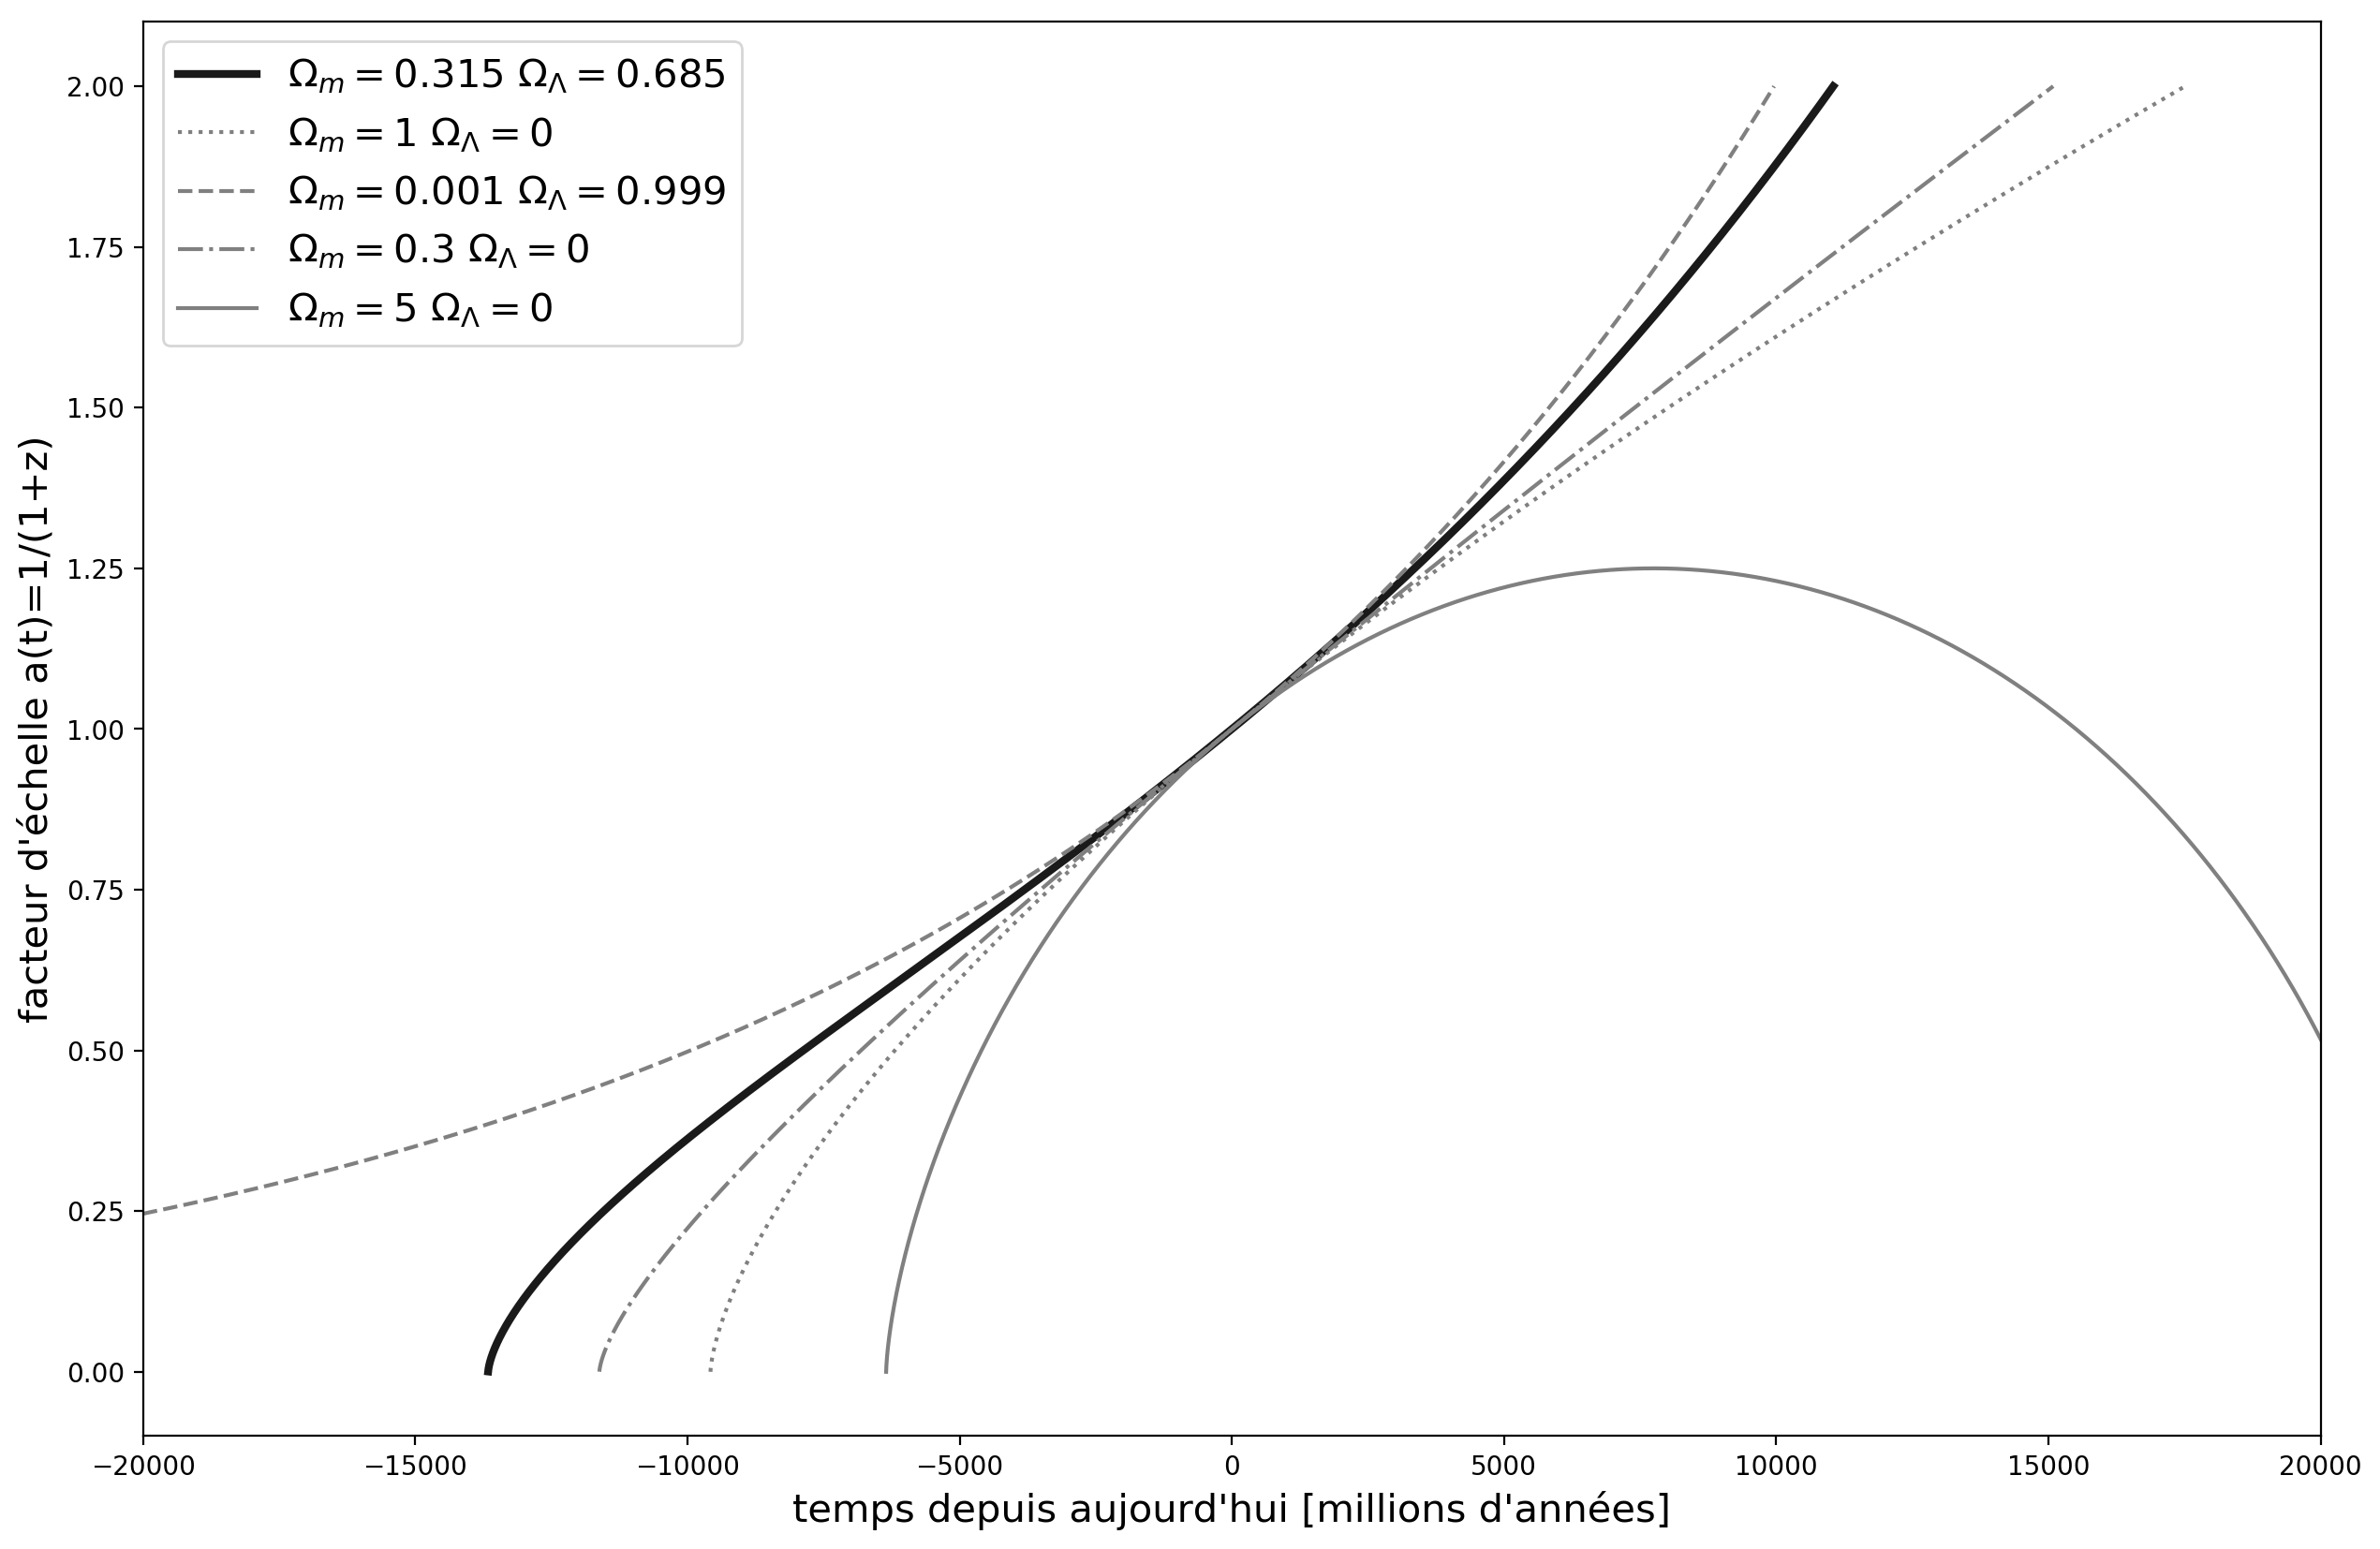
\includegraphics[height=10cm]{figs/a2t_cosmo.png}
	\caption[Facteur d'échelle pour différentes cosmologie]{Evolution temporelle du facteur d'échelle $a(t)$ pour différentes cosmologies. Ici om désigne le paramètre de densité de la matière et ov désigne celui de l'énergie noire. Notez que le facteur d'échelle est normalisé à 1 pour $t=0$.}
	\label{f:aexpcosmo}
\end{figure}

Le fait que l'Univers connaissent une phase d'expansion accélérée\index{accélération!expansion} n'est pas sans conséquences sur notre capacité future à faire de l'astrophysique et de la cosmologie. En effet actuellement, nous avons accès à des galaxies lointaines qui nous fuient, tandis que certaines galaxies proches sont actuellement en train de tomber sur nous et vont fusionner. De même, le rayonnement contribue peu au bilan énergétique de l'Univers mais reste détectable. Dans le futur, les galaxies lointaines vont échapper à nos télescopes~: trop lointaines, ou avec des vitesses de fuites trop grandes. Les galaxies proches auront fusionné avec nos systèmes locaux et nous n'auront qu'une 'méga' galaxie locale, peuplée d'un seul type d'étoile (vieilles et peu brillantes), dépourvue de gaz qui aura flambé lors des multiples fusions. Pour finir la densité de rayonnement deviendra inexorablement trop faible pour pouvoir être détectée, et les recherches actuelles faites sur le fond diffus cosmologique\index{fond diffus cosmologique} par exemple ne pourront avoir lieu. En résumé, nous sommes actuellement dans une époque 'bénie' pour faire de la cosmologie~: l'Univers futur sera 'ennuyant' et beaucoup moins propice à la compréhension des objets astrophysiques et à la cosmologie.